\newcommand{\figSNAFUMotivate}{
\begin{figure}[t]
	\centering
	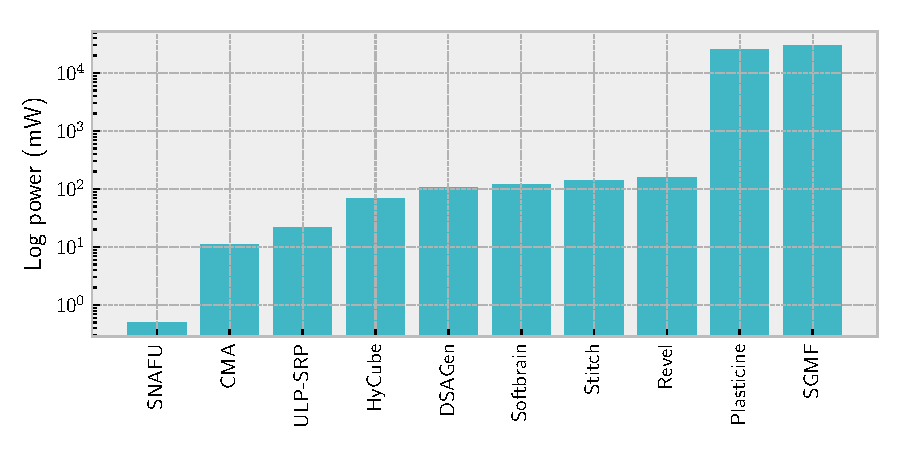
\includegraphics[width=\columnwidth]{snafu/figures/pdf/motivate.pdf}
	\caption{\snafuframe generates ultra-low-power CGRA fabrics that operate in a power regime not well explored by existing CGRAs.}
	\label{fig:motivate}
\end{figure}
}

\newcommand{\figSNAFUOverviewFramework}{
\begin{figure}[t]
	\centering
	\includegraphics[width=.65\columnwidth]{snafu/figures/pdf/overview.pdf}
	\caption{Overview of \snafu. \snafuframe is a flexible framework for generating ULP CGRAs. It takes a {\em bring-your-own functional unit} approach, allowing the designer to easily integrate custom logic tailored for specific domains.}
	\label{fig:overview:framework}
\end{figure}
}

\newcommand{\figSNAFUOverviewExecute}{
\begin{figure*}[t]
	\centering
	\includegraphics[width=\linewidth]{snafu/figures/pdf/execute.pdf}
	\caption{An example execution on a \snafuframe CGRA fabric. The DFG is extracted from vectorized C-code, compiled to a bitstream, and then executed according to asynchronous dataflow firing.}
	\label{fig:overview:execute}
\end{figure*}
}

\newcommand{\figSNAFUCompilation}{
\begin{figure}[htb]
	\centering
	\includegraphics[width=.9\columnwidth]{snafu/figures/pdf/compilation.pdf}
	\caption{Compiler extracts dataflow graphs from vectorized C-code and uses an integer linear program to optimally map the dataflow graph to specific PEs and routes in the CGRA fabric.}
	\label{fig:compilation}
\end{figure}
}

\newcommand{\figSNAFUArch}{
\begin{figure}[t]
	\centering
	\includegraphics[width=.65\columnwidth]{snafu/figures/pdf/arch.pdf}
	\caption{Architectural diagram of \snafuarch. \snafuarch possesses a RISC-V scalar core tightly coupled with the \snafuframe fabric. Both are attached to a unified 256\,KB banked memory.}
	\label{fig:arch}
\end{figure}
}

\newcommand{\figSNAFUPE}{
\begin{figure}[t]
	\centering
	\includegraphics[width=.65\columnwidth]{snafu/figures/pdf/pe.pdf}
	\caption{\snafuframe provides a standardized interface that makes integrating new types of PEs trivial. \snafuframe handles variable-latency logic, PE-specific configuration, and the sending and receiving of values from the on-chip network.}
	\label{fig:pe}
\end{figure}
}

\newcommand{\figSNAFUDie}{
\begin{figure}[t]
	\centering
	\includegraphics[width=.9\columnwidth]{snafu/figures/pdf/die.pdf}
	\caption{Layout of \snafuarch. Memory PEs are blue, scratchpad PEs are green, basic-ALU PEs are red, multiplier PEs are purple, the scalar core is yellow, and main-memory control logic is orange. The remaining grey regions contain routers and wires. }
	\label{fig:die}
\end{figure}
}

\newcommand{\figSNAFUPerf}{
\begin{figure}[htb]
	\centering
	\includegraphics[width=.9\columnwidth]{snafu/figures/pdf/perf-graph-crop.pdf}
	\caption{\snafu}
	\label{fig:perf:alone}
\end{figure}
}

\newcommand{\figSNAFUTopResults}{
	\begin{figure}[t]
		\centering
		\includegraphics[width=0.7\linewidth]{snafu/figures/pdf/energy_all_norm_legend-graph-crop.pdf}\\
		\vspace{0.4em}
		\begin{subfigure}{0.49\linewidth}
			\centering
			\includegraphics[width=0.8\linewidth]{snafu/figures/pdf/energy_avg-graph-crop.pdf}
			\caption{Energy savings.}
			\label{fig:top:energy}
		\end{subfigure}
		\begin{subfigure}{0.49\linewidth}
			\centering
			\includegraphics[width=0.8\linewidth]{snafu/figures/pdf/perf_overall-graph-crop.pdf}
			\caption{Avg performance.}
			\label{fig:top:perf}
		\end{subfigure}
		\caption{Average normalized energy and speedup (normalized to the scalar baseline). \snafuarch uses $81\%$ less energy and is $9.9\times$ faster than the scalar baseline.}
		\label{fig:top}	
	\end{figure}
}

\newcommand{\figSNAFUPrimaryResults}{
	\begin{figure*}[t]
		\centering
		\includegraphics[width=0.5\linewidth]{snafu/figures/pdf/energy_all_norm_legend-graph-crop.pdf}\\
		\vspace{0.4em}

		\begin{subfigure}{0.49\linewidth}
			\centering
			\includegraphics[width=\linewidth]{snafu/figures/pdf/energy_all_norm-graph-crop.pdf}
			\caption{Energy}
			\label{fig:energy:norm}
		\end{subfigure}
		\hfill
		\begin{subfigure}{0.5\linewidth}
			\centering
			\includegraphics[width=\linewidth]{snafu/figures/pdf/perf_all-graph-crop.pdf}
			\caption{Execution time}
			\label{fig:perf}
		\end{subfigure}
		\caption{Energy and execution time, normalized to the scalar baseline, across ten applications on large inputs. On average, \snafuarch uses $81\%$, $57\%$, $41\%$ less energy and is $9.9\times$, $3.2\times$, and $4.4\times$ faster than the scalar design, vector baseline, and \manic, respectively.
                }

		\label{fig:primary}
	\end{figure*}
}

\newcommand{\figSNAFUCacheNorm}{
\begin{figure}[htb]
	\centering
	\includegraphics[width=0.7\columnwidth]{snafu/figures/pdf/energy_all_norm_legend-graph-crop.pdf}\\
	\vspace{0.4em}
	\includegraphics[width=.9\columnwidth]{snafu/figures/pdf/cache_norm-graph-crop.pdf}
	\caption{\snafu}
	\label{fig:cache:norm:alone}
\end{figure}
}

\newcommand{\figSNAFUBufNorm}{
\begin{figure}[htb]
	\centering
	\includegraphics[width=0.7\columnwidth]{snafu/figures/pdf/energy_all_norm_legend-graph-crop.pdf}\\
	\vspace{0.4em}
	\includegraphics[width=.9\columnwidth]{snafu/figures/pdf/buf_norm-graph-crop.pdf}
	\caption{\snafu}
	\label{fig:buf:norm:alone}
\end{figure}
}

\newcommand{\figSNAFUInputEnergy}{
\begin{figure}[htb]
	\centering
	\includegraphics[width=.9\columnwidth]{snafu/figures/pdf/size_norm-graph-crop.pdf}
	\caption{\snafuarch}
	\label{fig:size:energy:alone}
\end{figure}
}

\newcommand{\figSNAFUInputPerf}{
\begin{figure}[htb]
	\centering
	\includegraphics[width=.9\columnwidth]{snafu/figures/pdf/size_perf-graph-crop.pdf}
	\caption{\snafuarch}
	\label{fig:size:perf:alone}
\end{figure}
}

\newcommand{\figSNAFUSensUnrollResults}{
\begin{figure*}[t]
	\centering
	\includegraphics[width=0.5\linewidth]{snafu/figures/pdf/energy_all_norm_legend-graph-crop.pdf}\\
	\vspace{0.4em}
	\begin{minipage}{0.31\linewidth}
		\begin{subfigure}[t]{0.49\linewidth}
			\centering
			\includegraphics[height=1in]{snafu/figures/pdf/sens_size_energy-graph-crop.pdf}
			\caption{Energy.}
			\label{fig:sens:size:energy}
		\end{subfigure}
		\hfill
		\begin{subfigure}[t]{0.49\linewidth}
			\centering
			\includegraphics[height=1in]{snafu/figures/pdf/sens_size_perf-graph-crop.pdf}
			\caption{Speedup.}
			\label{fig:sens:size:perf}
		\end{subfigure}
		\vspace{1.1em}
		\caption{\snafuarch vs.\ the scalar design across three input sizes -- small (S), medium (M) and large (L).}
		\label{fig:sens:size}
	\end{minipage}
        \hfill
	\begin{minipage}{0.67\linewidth}
		\begin{subfigure}[t]{0.49\columnwidth}
			\centering
			\includegraphics[width=0.99\linewidth]{snafu/figures/pdf/case_unroll_norm-graph-crop.pdf}
			\caption{Energy.}
			\label{fig:unroll:energy}
		\end{subfigure}
		\hfill
		\begin{subfigure}[t]{0.49\columnwidth}
			\centering
			\includegraphics[width=0.99\linewidth]{snafu/figures/pdf/case_unroll_perf-graph-crop.pdf}
			\caption{Speedup.}
			\label{fig:unroll:perf}
		\end{subfigure}
		\caption{Energy and speedup of \manic, un\manic (w/ loop unrolling), \snafuarch, and un\snafuarch (w/ loop unrolling), normalized to \snafuarch. un\snafuarch uses $31\%$ less energy and is $2.2\times$ faster \snafuarch; \manic benefits much less.}
		\label{fig:unroll}
	\end{minipage}
	\label{fig:sens}
\end{figure*}
}

\newcommand{\figSNAFUUnrollEnergy}{
\begin{figure}[htb]
	\centering
	\includegraphics[width=.9\columnwidth]{snafu/figures/pdf/case_unroll_norm-graph-crop.pdf}
	\caption{Energy}
\end{figure}
}

\newcommand{\figSNAFUUnrollPerf}{
\begin{figure}[htb]
	\centering
	\includegraphics[width=.9\columnwidth]{snafu/figures/pdf/case_unroll_perf-graph-crop.pdf}
	\caption{\snafuarch}
	\label{fig:unroll:perf:alone}
\end{figure}
}

\newcommand{\figSNAFUUnrollResults}{
	\begin{figure}[t]
		\centering
		\includegraphics[width=0.9\columnwidth]{snafu/figures/pdf/energy_all_norm_legend-graph-crop.pdf}\\
		\vspace{0.4em}
		\begin{subfigure}{0.49\columnwidth}
			\centering
			\includegraphics[width=\linewidth]{snafu/figures/pdf/case_unroll_norm-graph-crop.pdf}
			\caption{Energy.}
			\label{fig:unroll:energy}
		\end{subfigure}
		\hfill
		\begin{subfigure}{0.49\columnwidth}
			\centering
			\includegraphics[width=\linewidth]{snafu/figures/pdf/case_unroll_perf-graph-crop.pdf}
			\caption{Speedup.}
			\label{fig:unroll:perf}
		\end{subfigure}
		\caption{Energy and speedup of \manic, un\manic (w/ loop unrolling), \snafuarch, and un\snafuarch (w/ loop unrolling), normalized to \snafuarch. un\snafuarch uses $31\%$ less energy and is $2.2\times$ faster \snafuarch; \manic benefits much less.}
		\label{fig:unroll}
	\end{figure}
}

\newcommand{\figSNAFUAccel}{
	\begin{figure*}[t]
		\centering
		\includegraphics[width=.5\linewidth]{snafu/figures/pdf/case_dmm_energy_legend-graph-crop.pdf}\\
		\vspace{0.4em}

		\begin{subfigure}{0.32\linewidth}
			\centering
			\includegraphics[width=\linewidth]{snafu/figures/pdf/case_dmm_annotated-crop.pdf}
			\caption{DMM energy.}
			\label{fig:accel:dmm}
		\end{subfigure}
		\begin{subfigure}{0.32\linewidth}
			\centering
			\includegraphics[width=\linewidth]{snafu/figures/pdf/case_sort_annotated-crop.pdf}
			\caption{Sort energy.}
			\label{fig:accel:sort}
		\end{subfigure}
		\begin{subfigure}{0.32\linewidth}
			\centering
			\includegraphics[width=\linewidth]{snafu/figures/pdf/case_fft_annotated-crop.pdf}
			\caption{FFT energy.}
			\label{fig:accel:fft}
		\end{subfigure}

		\caption{Quantifying the cost of \snafu's programmability on three benchmarks. Each subfigure shows, from left-to-right, the effect of gradually removing \snafuarch's programmability and increasing its specialization, culminating in a hand-coded ASIC. Overall, \snafuarch's energy is within $2.6\times$ on average of the ASICs', and can be easily specialized to narrow the gap at low upfront design cost.}
		\label{fig:accel}
	\end{figure*}
}

\newcommand{\figSNAFUScratchEnergy}{
\begin{figure}[t]
	\centering
	\includegraphics[width=.9\columnwidth]{snafu/figures/pdf/case_scratch_norm-graph-crop.pdf}
	\caption{\snafuarch}
	\label{fig:scratch:energy:alone}
\end{figure}
}

\newcommand{\figSNAFUScratchPerf}{
\begin{figure}[htb]
	\centering
	\includegraphics[width=.9\columnwidth]{snafu/figures/pdf/case_scratch_perf-graph-crop.pdf}
	\caption{\snafuarch}
	\label{fig:scratch:perf:alone}
\end{figure}
}

\newcommand{\figSNAFUScratchResults}{
	\begin{figure}[t]
		\centering
		\includegraphics[width=0.9\columnwidth]{snafu/figures/pdf/energy_all_norm_legend-graph-crop.pdf}\\
		\vspace{0.4em}
		\begin{subfigure}{0.49\columnwidth}
			\centering
			\includegraphics[width=\linewidth]{snafu/figures/pdf/case_scratch_norm-graph-crop.pdf}
			\caption{Energy.}
			\label{fig:scratch:energy}
		\end{subfigure}
		\hfill
		\begin{subfigure}{0.49\columnwidth}
			\centering
			\includegraphics[width=\linewidth]{snafu/figures/pdf/case_scratch_perf-graph-crop.pdf}
			\caption{Speedup.}
			\label{fig:scratch:perf}
		\end{subfigure}
		\caption{Energy and speedup of \manic, \snafuarch w/ and w/out scratchpads, normalized to \snafuarch. Scratchpads improve energy-efficiency by $34\%$ and performance by $13\%$.}
		\label{fig:scratch}
	\end{figure}
}

\newcommand{\tabSNAFUParams}{
  \begin{table}
    %% \renewcommand{\tabSNAFUcolsep}{12pt}
%% \footnotesize
\centering
%% \resizebox{\linewidth}{!}{
\begin{tabular}{ccp{1.5in}r}
\toprule
 &  & \textbf{Parameter}       & \textbf{Values} \\
\midrule
 &  & Frequency		       & 50 MHz          \\
 &  & Main memory              & 256\,KB         \\
 &  & Scalar register \#       & 16		 \\[.5ex]
\midrule
\multirow{3}{.5em}{\rotatebox{90}{Vector}}
 &  & Vector register \#       & 16              \\
 &  & Vector length            & 16/32/64        \\
 &  & Window size (for \manic) & 8               \\[.5ex]
\midrule
\multirow{5}{.5em}{\rotatebox{90}{\snafuarch}}
 &  & Fabric dimensions	       & 6$\times$6	 \\
 &  & Memory PE \#    	       & 12		 \\
 &  & Basic-ALU PE \#          & 12		 \\
 &  & Multiplier PE \#         & 4		 \\
 &  & Scratchpad PE \#         & 8		 \\[.5ex]
\bottomrule
\end{tabular}
%}
\caption{Microarchitectural parameters.}
\label{tab:params}
\end{table}
}

\newcommand{\tabSNAFUApp}{
  \begin{table}[t]
\footnotesize
\centering
\resizebox{\linewidth}{!}{
\begin{tabular}{lp{1.25in}p{0.3in}p{0.3in}p{0.325in}}
\toprule
\textbf{Name} & \textbf{Description}                                      & \textbf{Small}                    & \textbf{Medium}                   & \textbf{Large}                    \\
\midrule
\bf FFT       & 2D Fast-fourier transform                                 & 16$\times$16                      & 32$\times$32                      & 64$\times$64                      \\
\bf DWT       & 2D Discrete wavelet trnsfrm                               & 16$\times$16                      & 32$\times$32                      & 64$\times$64                      \\
\bf Viterbi   & Viterbi decoder                                           & 256                               & 1024                              & 4096                              \\
\bf Sort      & Radix sort                                                & 256                               & 512                               & 1024                              \\
\bf SMM       & Sparse matrix-matrix                                      & 16$\times$16                      & 32$\times$32                      & 64$\times$64                      \\
\bf DMM       & Dense matrix-matrix                                       & 16$\times$16                      & 32$\times$32                      & 64$\times$64                      \\
\bf SMV       & Sparse matrix-dense vector                                & 32$\times$32                      & 64$\times$64                      & 128$\times$128                    \\
\bf DMV       & Dense matrix-dense vector                                 & 32$\times$32                      & 64$\times$64                      & 128$\times$128                    \\
\bf Sconv     & Sparse 2D convolution \newline \mbox{}\quad {\em filter:} & 16$\times$16, \newline 3$\times$3 & 32$\times$32, \newline 5$\times$5 & 64$\times$64, \newline 5$\times$5 \\
\bf Dconv     & Dense 2D convolution \newline \mbox{}\quad {\em filter:}  & 16$\times$16, \newline 3$\times$3 & 32$\times$32, \newline 5$\times$5 & 64$\times$64, \newline 5$\times$5 \\
\bottomrule
\end{tabular}
}
\caption{Benchmarks and their input sizes.}
\label{tab:app}
  \end{table}
}

\newcommand{\tabSNAFUTabs}{
	\tabSNAFUParams
	\tabSNAFUApp
}

\newcommand{\figSNAFUIntroOverview}{
	\begin{figure}
		\centering
		\includegraphics[width=0.75\linewidth]{snafu/figures/pdf/intro.pdf}
		\caption{\snafuframe is an ULP CGRA-generation framework and architecture. It converts a flexible abstract specification of a CGRA to synthesizable RTL. \snafuarch is an instantiation that integrates a $6\times6$ \snafuframe fabric with an ULP core and on-chip memory.}
		\label{fig:intro:overview}
	\end{figure}
}  

\newcommand{\figSNAFUIntroLayout}{
	\begin{figure}
		\centering
	        \includegraphics[width=.7\columnwidth]{snafu/figures/pdf/die.pdf}
	        \caption{Layout of \snafuarch, a complete ULP system with CGRA.}
	        \label{fig:intro:layout}
	\end{figure}
}  

\newcommand{\figSNAFUIntro}{
\begin{figure}[t]
	\centering
	\begin{subfigure}{0.49\linewidth}
		\centering
		\includegraphics[width=0.9\linewidth]{snafu/figures/pdf/energy_overall-graph-crop.pdf}
		\caption{Energy savings.}
		\label{fig:intro:energy}
	\end{subfigure}
	\begin{subfigure}{0.49\linewidth}
		\centering
		\includegraphics[width=0.9\linewidth]{snafu/figures/pdf/perf_overall-graph-crop.pdf}
		\caption{Performance.}
		\label{fig:intro:perf}
	\end{subfigure}

	\caption{\snafuarch's energy and performance normalized to a scalar baseline. On average, \snafuframe uses $81\%$ less energy and is $9.9\times$ faster, or $41\%$ less energy and $4.4\times$ faster than \manic.}
	\label{fig:intro}
\end{figure}	
}

\newcommand{\tabSNAFUMotivate}{
  \begin{table*}
  \centering
  \scriptsize
  \resizebox{\linewidth}{!}{
  \begin{tabular}{l|p{0.7in}p{0.7in}p{0.7in}|p{0.7in}p{0.7in}p{0.7in}|p{0.7in}}
    \toprule
                            & \multicolumn{3}{c|}{\bf Ultra-low-power CGRAs} & \multicolumn{3}{c|}{\bf High-performance CGRAs}                                                                                                                                                     \\[.5ex]
                            & \bf ULP-SRP~\cite{srp}                         & \bf CMA~\cite{cma} & \bf IPA~\cite{ipa} & \bf HyCube~\cite{karunaratne2017hycube} & \bf Revel~\cite{weng2020hybrid}    & \bf SGMF~\cite{voitsechov2014single} & \bf \snafu                            \\
    \midrule
    \bf Fabric size         & 3$\times$3                                     & 8$\times$10        & 4$\times$4         & 4$\times$4                              & 5$\times$5                         & 8$\times$8 + 32 mem                  & N$\times$N (6$\times$6 in \snafuarch) \\[.5ex]
    \bf NoC                 & Neighbors only                                 & Neighbors only     & Neighbors only     & Static, bufferless, multi-hop           & Static \& dynamic NoCs (2$\times$) & Dynamic routing                      & Static, bufferless, multi-hop       \\[.5ex]
    \bf PE assignment       & Static                                         & Static             & Static             & Static                                  & Static \emph{or} dynamic           & Dynamic                              & Static                              \\[.5ex]
    \bf Time-share PEs?     & Yes                                            & Yes                & Yes                & Yes                                     & Yes                                & Yes                                  & No                                  \\[.5ex]
    \bf PE firing           & Static                                         & Static             & Static             & Static                                  & Static \emph{or} dynamic           & Dynamic                              & Dynamic                             \\[.5ex]
    \bf Heterogeneous PEs?  & No                                             & No                 & No                 & No                                      & Yes                                & Yes                                  & Yes                                 \\[.5ex]
    \bf Buffering (approx.) & ---                                            & ---                & 188\,B / PE        & 272\,B / PE                             & $\approx$1\,KB / PE                & $\gg$1\,KB / PE                      & 40\,B / PE                          \\[.5ex]
    \midrule
    \bf Power               & 22\,mW                                         & 11\,mW             & 3--5\,mW           & 15--70\,mW                              & 160\,mW                            & 20\,W                                & $<$1\,mW                            \\[.5ex]
    \bf MOPS/mW (approx.)   & 30--100                                        & 100--200           & 140                & 60--90                                  & 60                                 & 60                                   & 305                                 \\[.5ex]
    \bottomrule
  \end{tabular}}
  \caption{Architectural comparison of \snafu to several prior CGRAs.}
  \label{tab:motivation}
\end{table*}
}
